\documentclass{bmstu}

\bibliography{biblio}

\renewcommand\labelitemi{---}
\renewcommand\labelitemii{---}

\usepackage{tabularray}

\usepackage{enumitem}

\usepackage{biblatex}
\setenumerate[1]{label=\arabic*)}

\newcommand{\specialcell}[2][c]{%
	\begin{tabular}[#1]{@{}c@{}}#2\end{tabular}}

% \usepackage[T1,T2A]{fontenc}    % Поддержка кириллицы
% \usepackage[utf8]{inputenc}     % Кодировка документа

% \usepackage{listingsutf8}
% \lstset{columns=fixed,basicstyle=\small,breaklines=true,inputencoding=utf8,keywordstyle=\bfseries\underbar,frame=single,tabsize=2,xleftmargin=20pt,xrightmargin=5pt}
% \lstset{extendedchars=true}
% \lstset{numbers=left,numberstyle=\small}

\geometry{a4paper,left=3.1cm,right=1.1cm,
    top=2cm,bottom=2cm,bindingoffset=0cm}

\usepackage{pdfpages}

\setlength{\parindent}{1.25cm}

\usepackage{ragged2e}
\justifying

\begin{document}

\makecourseworktitle{Информатика и системы управления}{Программное обеспечение ЭВМ и информационные технологии}{Разработка компилятора языка Lua}{Карпова~Е.~О./ИУ7-22М}{Ступников~А.~А.}{}{}{}

%Аналит: формализовать варианты использования и предоставляемые сервисом возможности и на их основе провести сравнительный анализ предложенного решения относительно существующих; формализовать и описать информацию, подлежащую хранению в БД и составить ER-диаграмму сущностей проектируемой БД в нотации Чена;
%Конструкт: спроектировать сущности БД и накладываемые ограничения целостности; описать проектируемую ролевую модель на уровне БД и определить права доступа к внутренним структурам;
%Технол: обосновать выбор средств реализации БД и приложения; описать интерфейс доступа к БД;
%Исслед: сравнительный анализ различных СУБД для хранения и обработки аналитических данных.

% 
\includepdf[pages={1}]{title.pdf}

% \begin{essay}{}

\par \textbf{Ключевые слова:} Компилятор, Lua, Go, ANTLR4, LLVM, IR.

\par Объектом разработки является компилятор языка Lua.

% \par В процессе разработки был проведён анализ предметной области и сравнительный анализ предложенного решения относительно существующих. Формализованы варианты использования, хранимые данные и предоставляемые сервисом возможности. Проведён выбор модели данных, базы данных по способу хранения и системы управления базой данных по способу доступа к базе данных. Составлена ER-диаграмма сущностей проектируемой базы данных в нотации Чена и спроектированы сущности базы данных и накладываемые ограничения целостности. Была описана проектируемая ролевая модель на уровне базы данных, определены права доступа к внутренним структурам и обоснован выбор средств реализации базы данных и приложения. Описан интерфейс доступа к базе данных. Также, проведено исследование производительности строковых и колоночных СУБД на агрегационных запросах.

% \par По результатам исследования сформулирован вывод о большей производительности колоночных баз данных по сравнению со строковыми для выполнения агрегационных запросов.

\end{essay}

\maketableofcontents

% \begin{definitions}
	\definition{Статический сервер}{сервер, возвращающий клиенту файлы, хранящиеся на диске, не изменяя содержимого этих файлов~\cite{елизаров2021автоматизированная}.}
	
	\definition{Сокет}{абстакция конечной точки соединения~\cite{ryaznu}.}
	
	\definition{Протокол}{набор соглашений логического уровня~\cite{tikh}.}
\end{definitions}
% \begin{abbreviations}
	\definition{HTTP}{HyperText Transfer Protocol~\cite{fielding2022rfc}.}
	\definition{TCP}{Transmission Control Protocol~\cite{eddy2022rfc}.}
	\definition{UDP}{User Datagram Protocol~\cite{tcp}.}
\end{abbreviations}

\chapter*{ВВЕДЕНИЕ}
\addcontentsline{toc}{chapter}{ВВЕДЕНИЕ}

В последние годы информационные технологии проникают всё в большее количество сфер общественной жизни, в том числе и сегмент торговли. Большинство современных компаний нацелено на продвижение именно своих интернет-платформ, что связано с уменьшением транзакционных расходов и ростом роли дистанционного взаимодействия~\cite{bib1}. Продвижение онлайн-площадок в сети Интернет при помощи рекламной рассылки является одним из распространённых методов~\cite{bib4}.

Целью данной работы является разработка базы данных для сервиса по почтовой рассылке персонализированных предложений.

В ходе работы необходимо решить следующие задачи:
\begin{enumerate}
	\item Провести анализ предметной области и сравнить предложенное решение с существующими.
	\item Формализовать варианты использования и предоставляемые сервисом возможности и описать информацию, подлежащую хранению в базе данных.
	\item Произвести выбор модели данных, базы данных по способу хранения и системы управления базой данных по способу доступа к базе данных.
	\item Составить ER-диаграмму сущностей проектируемой базы данных в нотации Чена и спроектировать сущности базы данных и накладываемые ограничения целостности.
	\item Описать проектируемую ролевую модель на уровне базы данных и определить права доступа к внутренним структурам.
	\item Описать выбор средств реализации базы данных и приложения и  интерфейс доступа к базе данных.
	\item Провести сравнительный анализ различных систем управления базой данных для хранения и обработки аналитических данных.
\end{enumerate}
\chapter{Аналитический раздел}

%\par В этом разделе будет проведён анализ предментой области и обзор существующих решений, обоснована актуальность решаемой продуктом задачи. Также, будет формализована задача, пользовательские сценарии, данные и выбрана модель данных, тип базы данных и тип системы управления базой данных. 

\section{Устройство компилятора}

Процесс компиляции состоит из следующих этапов~\cite{compilers}.
\begin{enumerate}
	\item Лексический анализ. 
	\item Синтаксический анализ. 
	\item Семантический анализ.
	\item Генерация кода на языке целевой платформы.
\end{enumerate}

\section{Лексический анализатор}

Лексический анализ~---~распознавание базовых элементов языка, перевод исходной программы в поток лексем и передача токенов, образуемых этими лексемами, последующим стадиям компиляции.


Основные функции лексического анализатора:
\begin{itemize}
	\item удаление пробелов и комментариев, обнаружение лексических ошибок;
	\item сборка последовательности цифр, формирующих константу;
	\item распознавание идентификаторов и ключевых слов.
\end{itemize}

\begin{table}[h!]
	\centering
	\begin{tabular}{p{1\linewidth}}
	  \centering
	  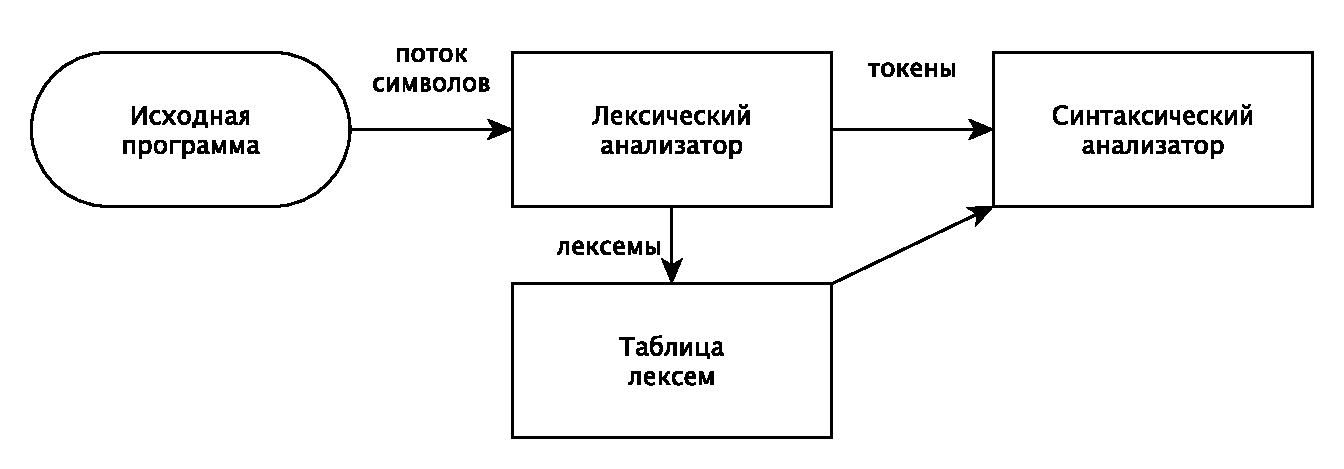
\includegraphics[width=0.8\linewidth]{./images/lexer.pdf}
	  \captionof{figure}{Лексический анализатор}
	  \label{img:lexer}
	\end{tabular}
  \end{table}

\section{Синтаксический анализатор}

Вторая фаза компилятора~---~синтаксический анализ или разбор. Анализатор использует первые компоненты токенов, полученных при лексическом анализе, для создания древовидного промежуточного представления, которое описывает грамматическую структуру потока токенов. 
Типичным представлением является синтаксическое дерево.

Полученная грамматическая структура используется в последующих этапах компиляции для анализа исходной программы и генерации кода для целевой платформы.
Синтаксический анализ выявляет синтаксические ошибки, относящиеся к нарушению структуры программы.

\begin{table}[h!]
	\centering
	\begin{tabular}{p{1\linewidth}}
	  \centering
	  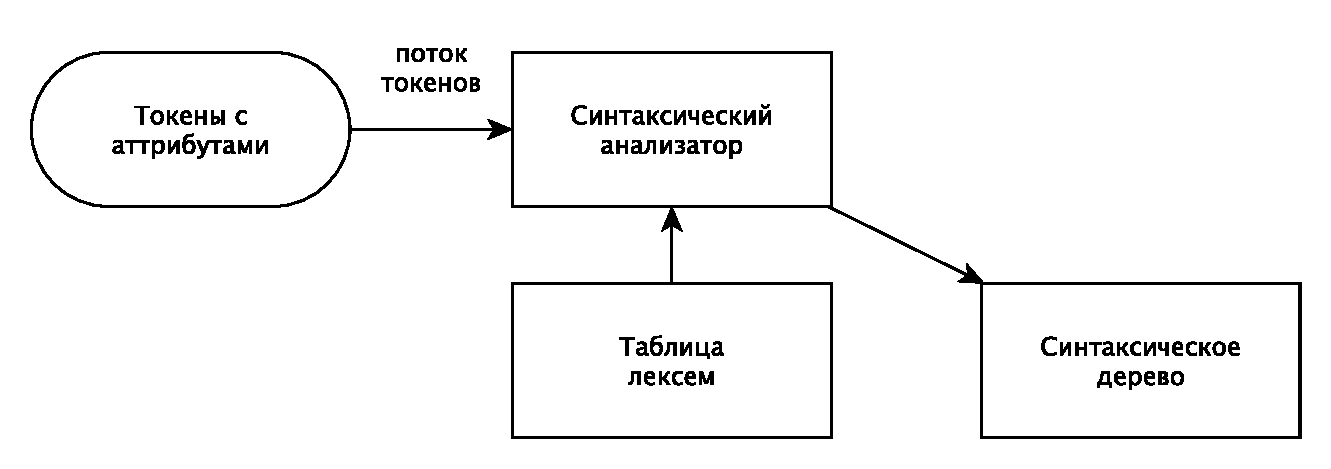
\includegraphics[width=0.8\linewidth]{./images/syntax.pdf}
	  \captionof{figure}{Синтаксический анализатор}
	  \label{img:syntax}
	\end{tabular}
  \end{table}

\section{Семантический анализатор}

Семантический анализатор использует синтаксическое дерево и информацию из таблицы символов для проверки исходной программы на семантическую согласованность с определением языка. Он также собирает информацию о типах и сохраняет все в синтаксическом дереве или в таблице символов для последующего использования в процессе генерации промежуточного кода.

Важной частью семантического анализа является проверка типов, когда компилятор проверяет, имеет ли каждый оператор операнды соответствующего типа.

Как правило, семантический анализатор разделяется на ряд более мелких, каждый из которых предназначен для конкретной конструкции. Соответствующий семантический анализатор вызывается синтаксическим анализатором как только он распознает синтаксическую единицу, требующую обработки.

\begin{table}[h!]
	\centering
	\begin{tabular}{p{1\linewidth}}
	  \centering
	  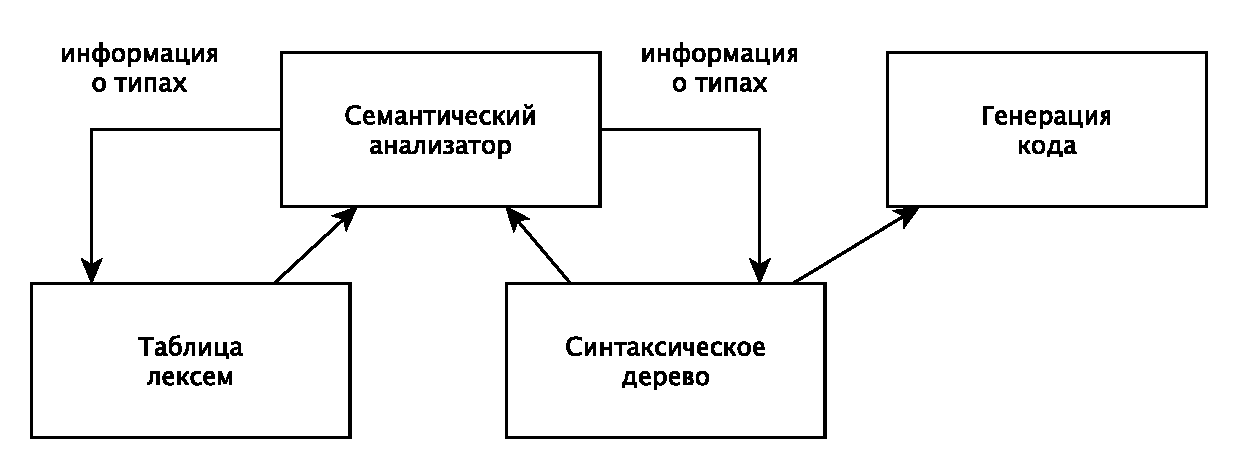
\includegraphics[width=0.8\linewidth]{./images/sem.pdf}
	  \captionof{figure}{Семантический анализатор}
	  \label{img:sem}
	\end{tabular}
  \end{table}

\section{Генерация кода}

\subsection{Генерация промежуточного кода}

В процессе трансляции исходной программы в целевой код компилятор может создавать одно или несколько промежуточных представлений различного вида.
Синтаксические деревья являются видом промежуточного представления. Обычно они используются в процессе синтаксического и семантического анализа.

После синтаксического и семантического анализа исходной программы многие компиляторы генерируют явное низкоуровневое или машинное промежуточное представление исходной программы, которое можно рассматривать как программу для абстрактной вычислительной машины. 
Такое промежуточное представление должно обладать двумя важными свойствами: оно должно легко генерироваться и легко транслироваться в целевой машинный язык.

\subsection{Оптимизация}

Фаза машинно-независимой оптимизации кода пытается улучшить промежуточный код, чтобы затем получить более качественный целевой код. Например, более быстрый код, короткий код, или код, использующий меньшее количество ресурсов. 

\subsection{Генерация кода на целевом языке}

Генератор кода получает в качестве входных данных промежуточное представление исходной программы и отображает его в целевой язык. 
Если целевой язык представляет собой машинный код, для каждой переменной, используемой программой, выбираются соответствующие регистры или ячейки памяти. 
Затем промежуточные команды транслируются в последовательности машинных команд, выполняющих те же действия.

\section{Таблица символов}

Важная функция компилятора состоит в том, чтобы записывать имена переменных в исходной программе и накапливать информацию о разных атрибутах каждого имени. 
Эти атрибуты могут предоставлять информацию о выделенной памяти для данного имени, его типе, области видимости и, в случае имен процедур, такие сведения, как количество и типы их аргументов, метод передачи каждого аргумента, а также возвращаемый тип.
Таблица символов представляет собой структуру данных, содержащую записи для каждого имени переменной, с полями для атрибутов имени. 

\section{Синтаксическое дерево}

Синтаксическое дерево~---~дерево, в котором каждый внутренний узел представляет операцию, а дочерние узлы~---~аргументы этой операции.
Порядок операций в дереве согласуется с обычными правилами, например, умножение имеет более высокий приоритет, чем сложение, и должно быть выполнено до сложения.

\begin{table}[h!]
	\centering
	\begin{tabular}{p{1\linewidth}}
	  \centering
	  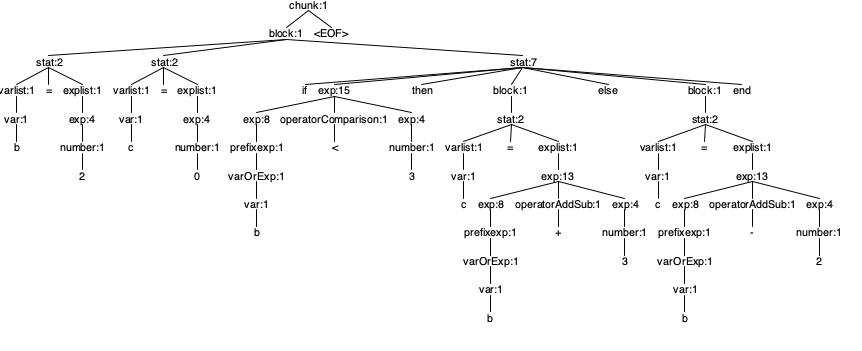
\includegraphics[width=1\linewidth]{./images/tree.png}
	  \captionof{figure}{Пример синтаксического дерева}
	  \label{img:tree}
	\end{tabular}
  \end{table}

\section{Генераторы лексических анализаторов}

Существует множество генераторов, наиболее популярные из них~---~Lex, Flex и ANTLR4.

Lex~---~стандартный инструмент для получения лексических анализаторов в операционных системах Unix~\cite{lesk1975lex}. 
В результате обработки входного потока получается исходный файл на языке C. 
Lex-файл разделяется на три блока: блок определений, правил и кода на C.

Flex заменяет Lex в системах на базе пакетов GNU и имеет аналогичную функциональность~\cite{sampath2007test}.

ANTLR (ANother Tool for Language Recognition)~---~генератор лексических и синтаксических анализаторов, позволяет создавать анализаторы на таких языках, как: Java, C\#, Go, C++ и других~\cite{parr2004s}.

ANTLR генерирует классы нисходящего рекурсивного синтаксического анализатора, на основе правил, заданных грамматикой. 
Он также позволяет строить и обходить деревья синтаксического анализа с использованием паттернов посетитель или слушатель. 
Благодаря своей эффективности и простоте использования, ANTLR является одним из наиболее предпочтительных генераторов анализаторов при создании кода синтаксического анализатора. 
В текущей работе было решено использовать этот инструмент.

\section{Генераторы синтаксических анализаторов}

Для создания синтаксических анализаторов используются такие инструменты, как Yacc/Bison, Coco/R и описанный ранее ANTLR.

Yacc~---~стандартный генератор синтаксических парсеров в Unix системах, Bison~---~аналогичный ему генератор для GNU систем~\cite{yacc}.

Coco/R~---~генератор лексических и синтаксических анализаторов~\cite{mossenbock2003compilergenerator}. 
Лексические анализаторы работают по принципу конечных автоматов, а синтаксические используют рекурсивный спуск. 
Поддерживаются такие языки программирования, как C\+\+, C\#, Java и другие.

\section{LLVM}

LLVM (Low Level Virtual Machine)~---~проект программной инфраструктуры для создания компиляторов и сопутствующих им утилит~\cite{sarda2015llvm}. 
В его основе лежит платформонезависимая система кодирования машинных инструкций~---~байткод LLVM IR. 
LLVM может создавать байткод для множества платформ, включая ARM, x86, x86-64, GPU от AMD и Nvidia и другие. 
Для компиляции LLVM IR в код платформы используется clang. 
В состав LLVM входит также интерпретатор LLVM IR, способный исполнять код без компиляции в код платформы.

LLVM поддерживает целые числа произвольной разрядности, числа с плавающей точкой, массивы, структуры и функции. 
Большинство инструкций в LLVM принимает два аргумента и возвращает одно значение.
Значения в LLVM определяются текстовым идентификатором. 
Тип операндов всегда указывается явно и однозначно определяет тип результата. 
Операнды арифметических инструкций должны иметь одинаковый тип, но сами инструкции «перегружены» для любых числовых типов и векторов.
LLVM IR строго типизирован, поэтому существуют операции приведения типов, которые явно кодируются специальными инструкциями. 
Кроме того, существуют инструкции преобразования между целыми числами и указателями, а также универсальная инструкция для приведения типов bitcast.
Значения в памяти адресуются типизированными указателями. 
Обратиться к ней можно с помощью двух инструкций: load и store. Инструкция alloca выделяет память на стеке. 
Она автоматически освобождается при выходе из функции.
Для вычисления адресов элементов массивов и структур с правильной типизацией используется инструкция getelementptr. 
Она только вычисляет адрес без обращения к памяти, принимает произвольное количество индексов и может разыменовывать структуры любой вложенности.

\section{Вывод}

В данном разделе приведён обзор основных фаз компиляции, описана каждая из них. 
Также был выбран генератор лексического и синтаксического анализаторов~---~ANTLR и LLVM в качестве генератора машинного кода.


















 

\chapter{Конструкторский раздел}

%В данном разделе будет проведена формализация сущностей проектируемой системы, описаны используемые домены, ролевая модель и реализуемая табличная функция.

\section{Концептуальная модель разрабатываемого компилятора}

Концептуальная модель разрабатываемого компилятора в нотации IDEF0 представлена на рисунке~\ref{idef0}.

\begin{figure}[H]
	\center{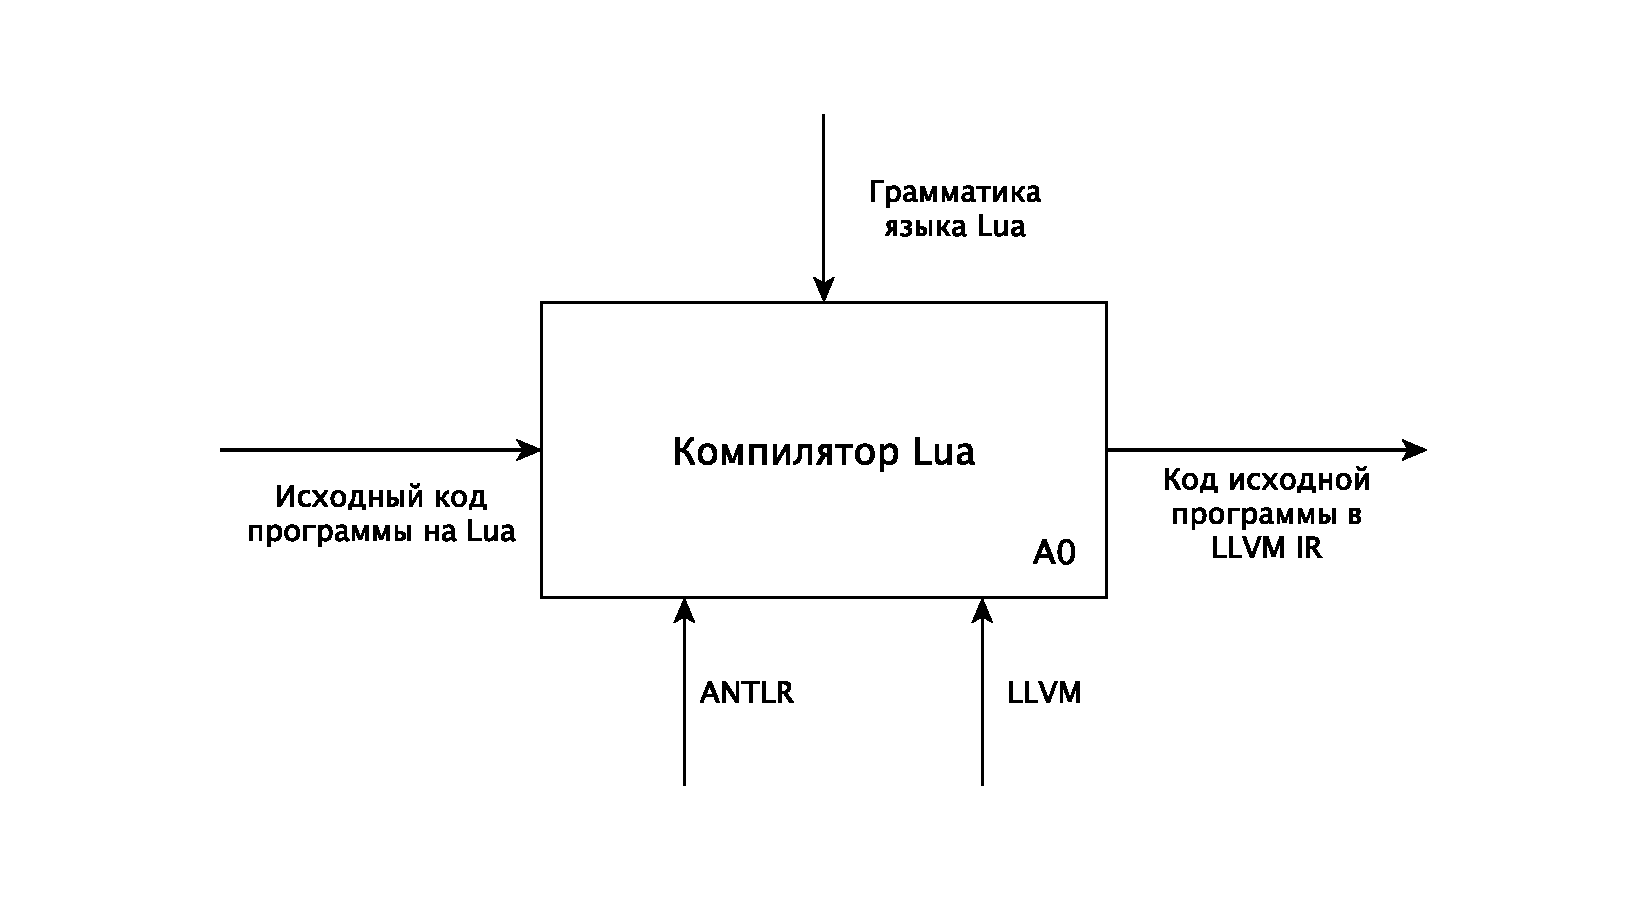
\includegraphics[width=0.8\linewidth]{./images/idef.pdf}}
	\caption{Концептуальная модель разрабатываемого компилятора в нотации IDEF0}
	\label{idef0}
   \end{figure}

\section{Язык Lua}

Lua~---~встраиваемый язык сценариев. 
Он поддерживает процедурное программирование, объектно-ориентированное программирование, функциональное программирование, программирование, управляемое данными, и описание данных.
Lua сочетает в себе процедурный синтаксис с конструкциями описания данных, основанными на ассоциативных массивах и расширяемой семантике. 
Lua динамически типизирован, работает путем интерпретации байт-кода с помощью виртуальной машины на основе регистров и имеет автоматическое управление памятью с инкрементальной сборкой мусора, что делает его идеальным для конфигурирования, написания сценариев и быстрого прототипирования.

Грамматика приведена в Приложении А.

\section{Лексический и синтаксический анализаторы}

Лексический и синтаксический анализаторы в данной работе генерируются с помощью ANTLR. 
На вход поступает грамматика языка в формате ANTLR4.

В результате работы создаются файлы, содержащие классы лексера и парсера, а также вспомогательные файлы и классы для их работы. 
Также генерируются шаблоны классов для обхода дерева разбора, которое получается в результате работы парсера.
На вход лексера подаётся текст программы, преобразованный в поток символов. 
На выходе получается поток токенов, который затем подаётся на вход парсера.
Результатом его работы является дерево разбора.
Ошибки, возникающие в ходе работы лексера и парсера, выводятся в стандартный поток ввода-вывода.

\section{Семантический анализ}

Абстрактное синтаксическое дерево можно обойти двумя способами: применяя паттерн Listener или Visitor.
Listener позволяет обходить дерево в глубину и вызывает обработчики соответствующих событий при входе и выходе из узла дерева.
Visitor предоставляет возможность более гибко обходить построенное дерево и решить, какие узлы и в каком порядке нужно посетить. 
Таким образом, для каждого узла реализуется метод его посещения. Обход начинается с точки входа в программу.
В данной работе используется паттерн Visitor.

\section{Вывод}

В текущем разделе была представлена концептуальная модель в нотации IDEF0, приведена грамматика языка Lua, описаны принципы работы лексического и синтаксического анализаторов и идея семантического анализа.

\chapter{Технологический раздел}

В данном разделе приведена реализация статического сервера.

\section{Листинг алгоритма работы статического \\ сервера}

В листинге \ref{lst:static_server} приведен программный код работы статического сервера.
 
\begin{lstlisting}[language=C, label=lst:static_server, caption={Листинг алгоритма работы статического сервера}]
void accept_connection() {
    int fd = accept(sockfd, NULL, NULL);
    if (fd < 0) {
        log_error("accept failed");
        return;
    }

    struct epoll_event e;
    e.events = EPOLLIN | EPOLLET;
    e.data.fd = fd;
    if (epoll_ctl(epollfd, EPOLL_CTL_ADD, fd, &e) < 0) {
        log_fatal("epoll_ctl: failed to add socket");
    }

    log_info("got new connection");
}

void use_fd(int fd) {
    char buf[BUF_SIZE] = {0};

    ssize_t n = read(fd, buf, sizeof(buf));
    if (n == 0) {
        log_info("connection is closed");
        return;
    }

    http_request_t req;
    req.fd = fd;
    int rc = http_parse_request(buf, &req);
    if (rc != OK) {
        log_error("cannot parse request: %s", error_messages[rc]);
        if (rc == ERR_UNSUPPORTED_METHOD) {
            http_write_error(&req, RESPONSE_CODE_METHOD_NOT_ALLOWED);
        }
        return;
    }

    rc = http_handle(&req);
    if (rc != OK) {
        log_error("cannot handle request: %s", error_messages[rc]);
        return;
    }

    log_debug("%s \"%s\"", http_methods_map[req.method], req.uri);
}

void *handle_connections(void *data) {
    int rc;

    log_debug("starting processing");

    struct epoll_event events[MAX_EVENTS];

    while (running) {
        int n = epoll_wait(epollfd, events, MAX_EVENTS, -1);
        if (n < 0) {
            if (!running) {
                break;
            }
            log_fatal("epoll failed");
        }

        for (int i = 0; i < n; i++) {
            if (events[i].data.fd == sockfd) {
                accept_connection();
                continue;
            }

            use_fd(events[i].data.fd);
        }
    }

    pthread_exit((void *) 0);
}
\end{lstlisting}

% \chapter{Исследовательский раздел}

Характеристики компьютера, на котором было проведено тестирование разработанного ПО: операционная система Debian Bookworm, версия ядра Linux 6.1.31.

На рисунке \ref{img:test} представлен пример отображения на дисплее информации о потребляемой процессом containerd виртуальной памяти.

\begin{table}[h!]
  \centering
  \begin{tabular}{p{1\linewidth}}
    \centering
    
\includegraphics[width=0.8\linewidth]{./images/test.pdf}
    \captionof{figure}{Пример отображения на дисплее информации о потребляемой процессом containerd виртуальной памяти}
    \label{img:test}
  \end{tabular}
\end{table}

На рисунках \ref{img:sfu}~--~\ref{img:mod} представлен пример отображения в системе специального файла устройства для разработанного драйвера и модуля ядра соответственно.

\begin{table}[h!]
  \centering
  \begin{tabular}{p{1\linewidth}}
    \centering
    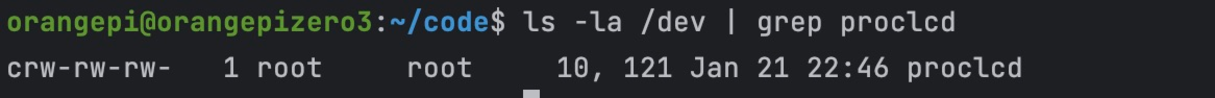
\includegraphics[width=0.9\linewidth]{./images/sfu.pdf}
    \captionof{figure}{Пример отображения в системе специального файла устройства для разработанного драйвера}
    \label{img:sfu}
  \end{tabular}
\end{table}

\begin{table}[h!]
  \centering
  \begin{tabular}{p{1\linewidth}}
    \centering
    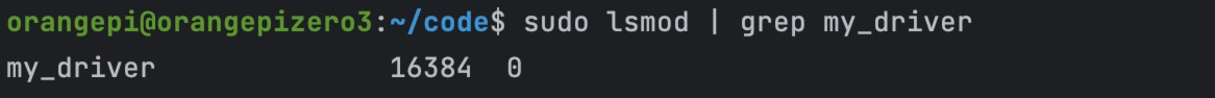
\includegraphics[width=0.9\linewidth]{./images/mod.pdf}
    \captionof{figure}{Пример отображения в системе модуля ядра}
    \label{img:mod}
  \end{tabular}
\end{table}

На рисунках \ref{img:out_init}~--~\ref{img:out_print} представлен пример логов разработанного модуля ядра при инициализации и в процессе вывода данных на дисплей соответственно.

\begin{table}[h!]
  \centering
  \begin{tabular}{p{1\linewidth}}
    \centering
    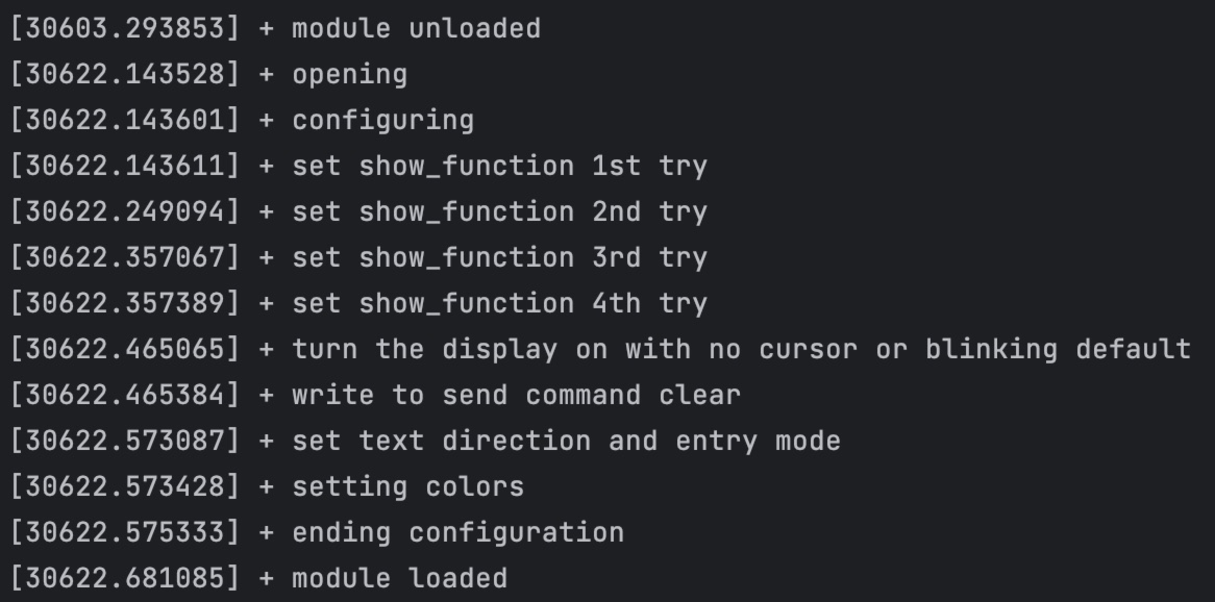
\includegraphics[width=0.8\linewidth]{./images/out_init.pdf}
    \captionof{figure}{Пример логов разработанного модуля ядра при инициализации}
    \label{img:out_init}
  \end{tabular}
\end{table}

\begin{table}[h!]
  \centering
  \begin{tabular}{p{1\linewidth}}
    \centering
    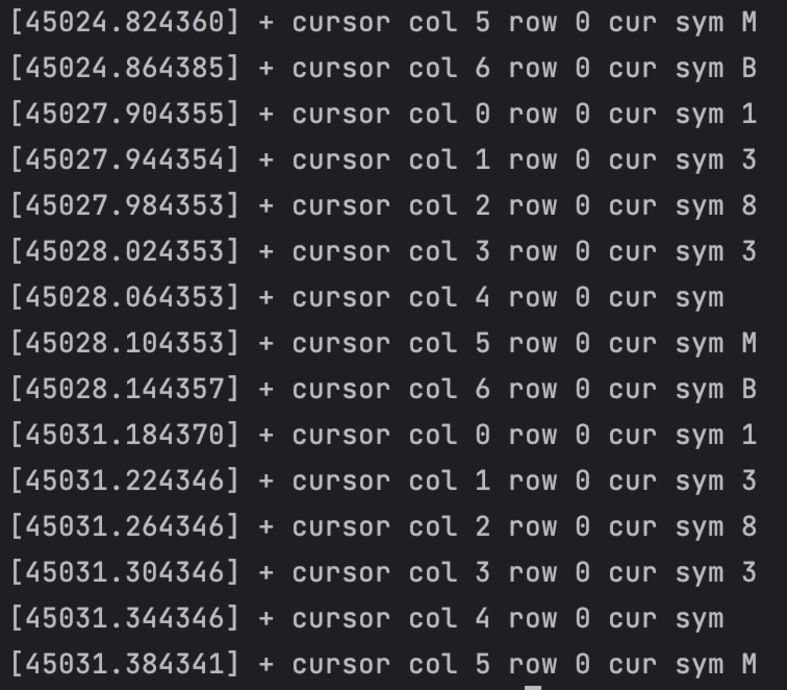
\includegraphics[width=0.6\linewidth]{./images/out_print.pdf}
    \captionof{figure}{Пример логов разработанного модуля ядра в процессе вывода данных на дисплей}
    \label{img:out_print}
  \end{tabular}
\end{table}

\newpage
На рисунке \ref{img:if} представлен интерфейс клиентской части приложения.
\newpage

\begin{table}[h!]
  \centering
  \begin{tabular}{p{1\linewidth}}
    \centering
    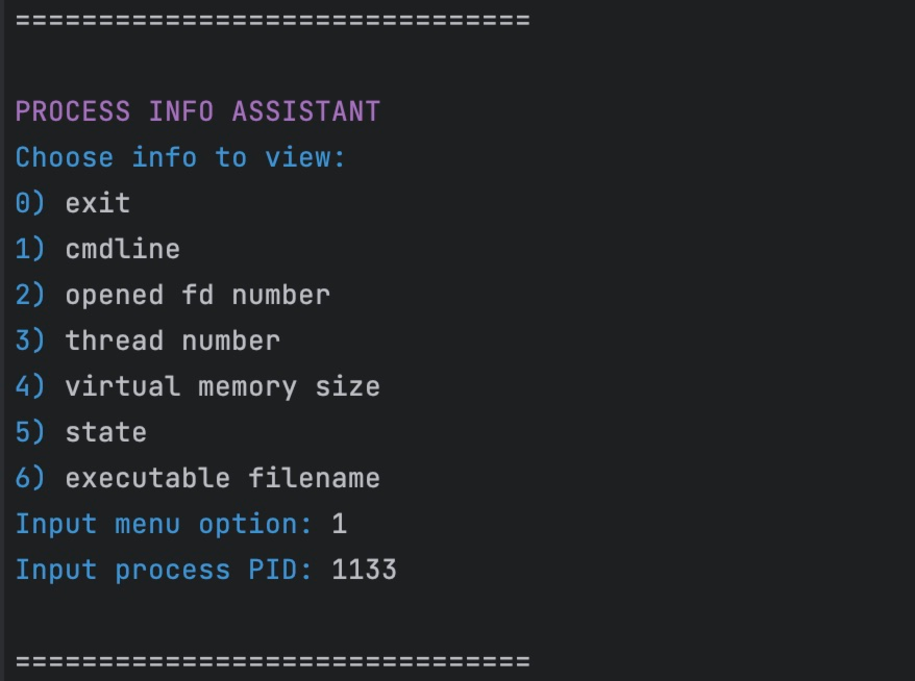
\includegraphics[width=0.7\linewidth]{./images/if.pdf}
    \captionof{figure}{Интерфейс клиентской части приложения}
    \label{img:if}
  \end{tabular}
\end{table}

\section*{Вывод}
Был представлен пример отображения информации о конкретном процессе на символьном дисплее. Также, были приведены примеры отображения в системе специального файла устройства, отображение модуля ядра, пример отладочного вывода разработанного модуля и вид пользовательского интерфейса.

\newpage

\chapter*{ЗАКЛЮЧЕНИЕ}
\addcontentsline{toc}{chapter}{ЗАКЛЮЧЕНИЕ}

В ходе выполнения курсовой работы были решены следующие задачи:
\begin{enumerate}
	\item Был проведён анализ предметной области и сравнение предложенного решения с существующими.
	\item Были формализованы варианты использования и предоставляемые сервисом возможности и описана информация, подлежащая хранению в базе данных.
	\item Был проведён выбор модели данных, базы данных по способу хранения и системы управления базой данных по способу доступа к базе данных.
	\item Была составлена ER-диаграмма сущностей проектируемой базы данных в нотации Чена и спроектированы сущности базы данных и накладываемые ограничения целостности.
	\item Была описана проектируемая ролевая модель на уровне базы данных и определены права доступа к внутренним структурам.
	\item Был обоснован выбор средств реализации базы данных и приложения и описан интерфейс доступа к базе данных.
	\item Был проведён сравнительный анализ различных систем управления базой данных для хранения и обработки аналитических данных.
\end{enumerate}

Таким образом, была достигнута цель работы: была разработана база данных для сервиса по почтовой рассылке персонализированных предложений.

В будущем разработанную программу можно будет усовершенствовать, добавив больше типов фильтрации, возможность анализировать действия клиентов с отправленными письмами и расширив функционал по редактированию шаблона рекламных писем.

\makebibliography

\begin{appendices}
	\chapter{Приложение А}
	Примеры работы реализации алгоритма шифрования машиной Enigma.
	
\begin{table}[H]
	\centering
	\begin{tabular}{p{1\linewidth}}
		\centering
		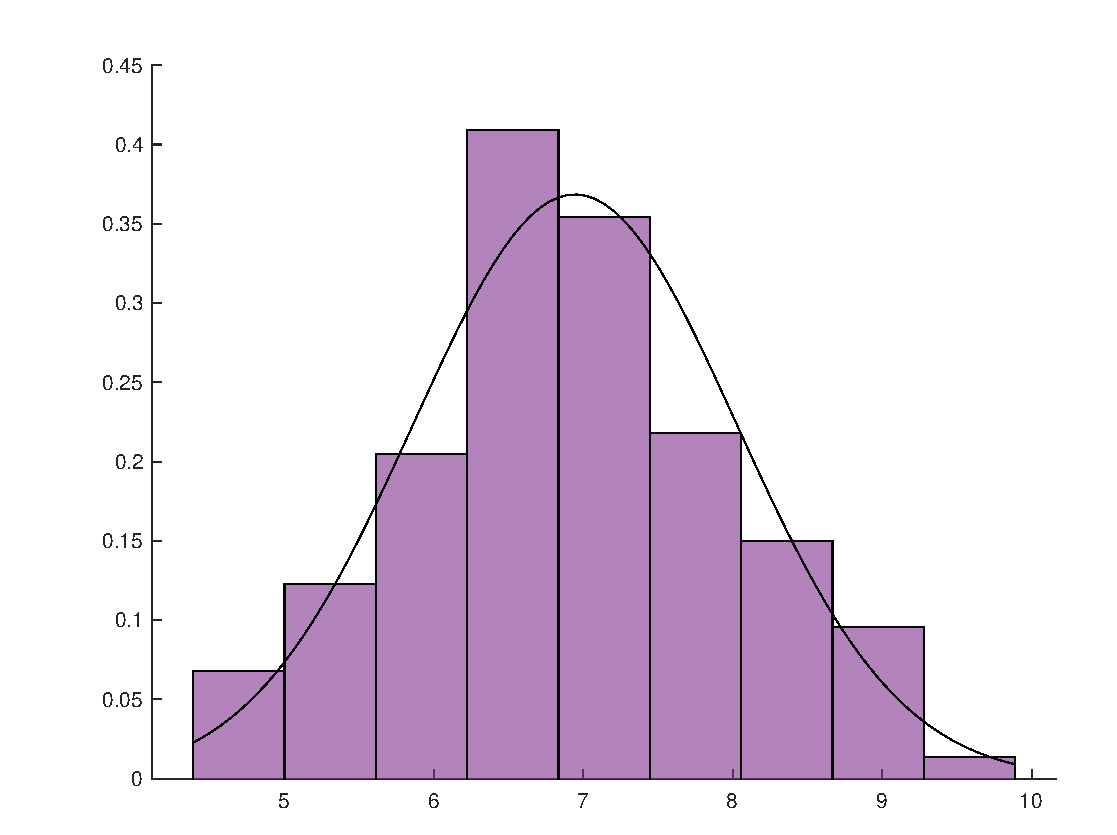
\includegraphics[width=0.9\linewidth]{inc/pdfs/1.pdf}
		\captionof{figure}{txt файл на русском}
		\label{img:enigma}
	\end{tabular}
\end{table}

\begin{table}[H]
	\centering
	\begin{tabular}{p{1\linewidth}}
		\centering
		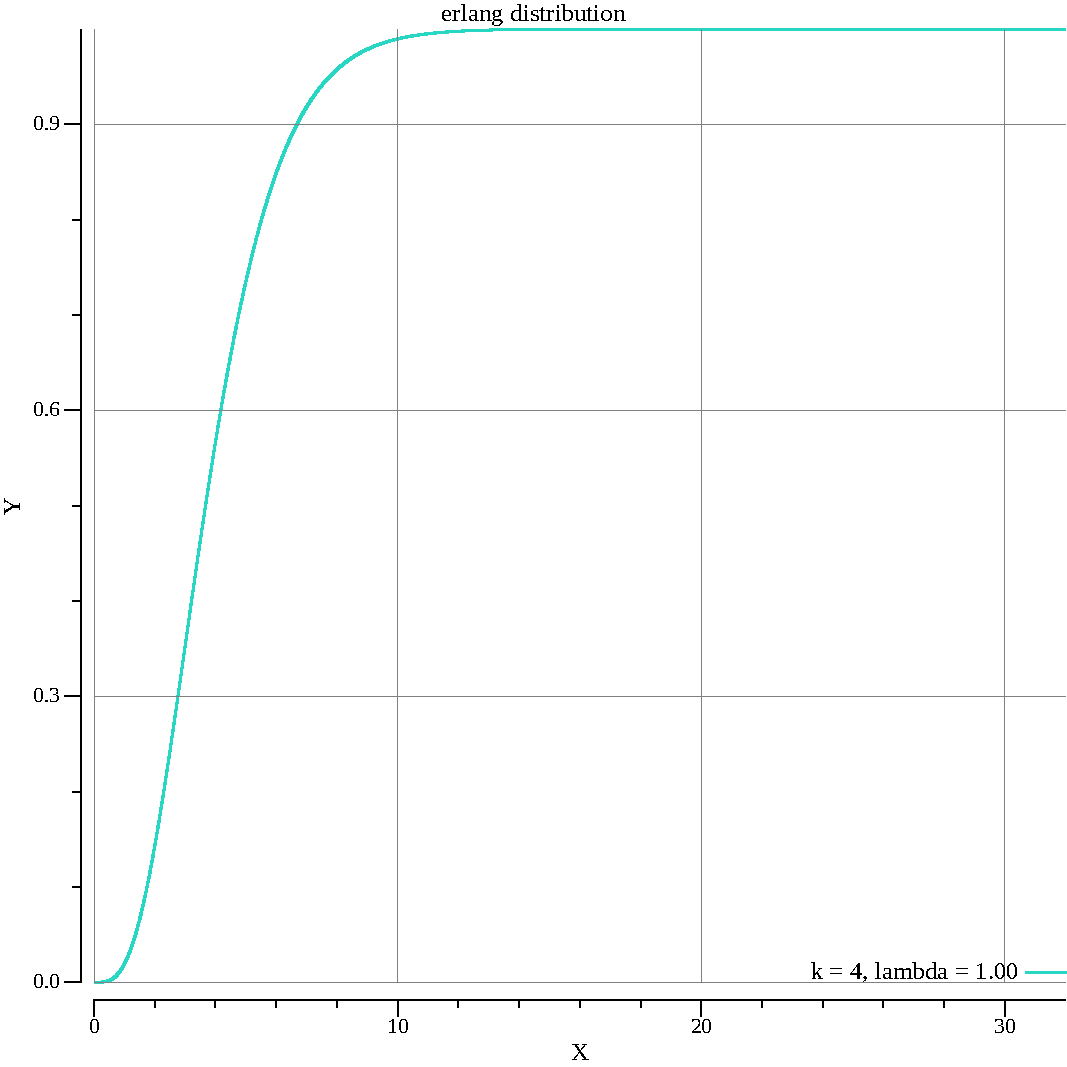
\includegraphics[width=0.9\linewidth]{inc/pdfs/2.pdf}
		\captionof{figure}{txt файл на английском}
		\label{img:enigma}
	\end{tabular}
\end{table}

\begin{table}[H]
	\centering
	\begin{tabular}{p{1\linewidth}}
		\centering
		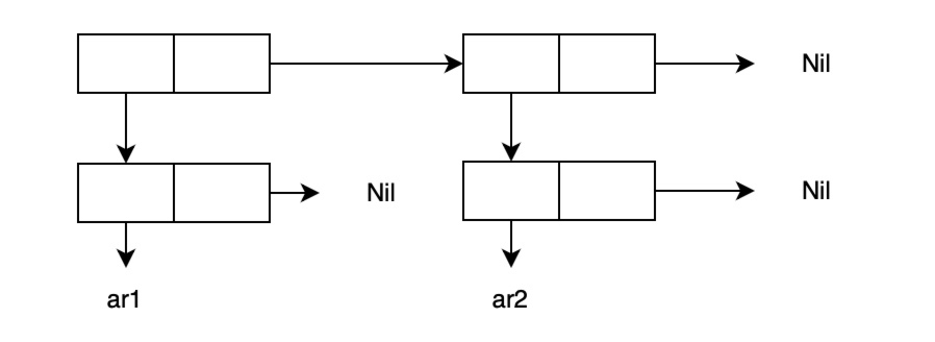
\includegraphics[width=0.9\linewidth]{inc/pdfs/3.pdf}
		\captionof{figure}{Пустой файл}
		\label{img:enigma}
	\end{tabular}
\end{table}

\begin{table}[H]
	\centering
	\begin{tabular}{p{1\linewidth}}
		\centering
		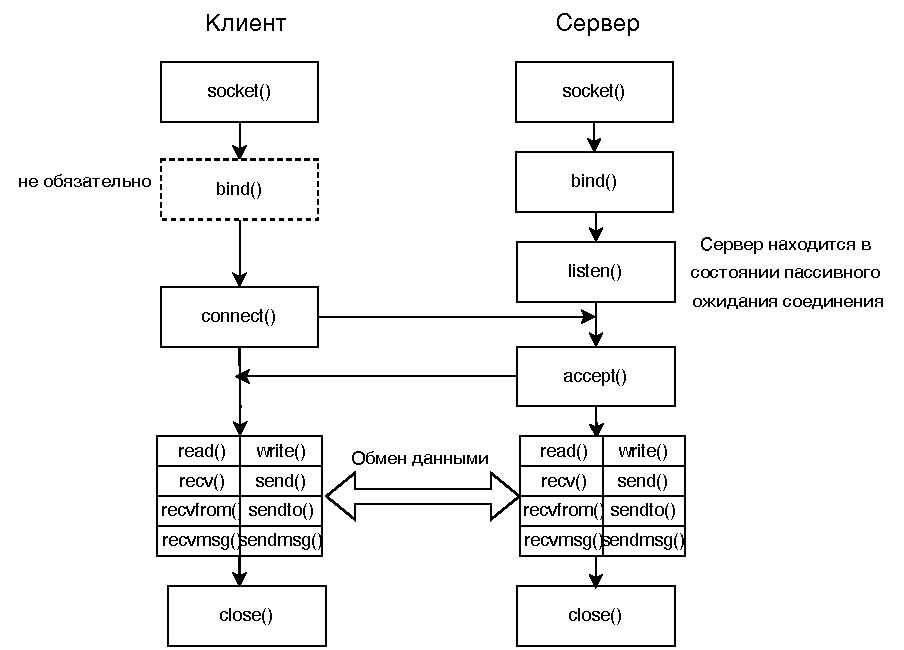
\includegraphics[width=0.9\linewidth]{inc/pdfs/4.pdf}
		\captionof{figure}{zip архив с двумя файлами}
		\label{img:enigma}
	\end{tabular}
\end{table}

\begin{table}[H]
	\centering
	\begin{tabular}{p{1\linewidth}}
		\centering
		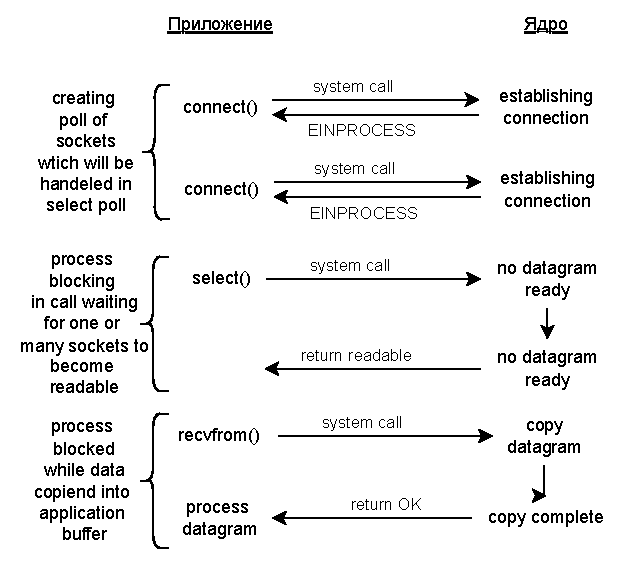
\includegraphics[width=0.9\linewidth]{inc/pdfs/5.pdf}
		\captionof{figure}{jpg изображение}
		\label{img:enigma}
	\end{tabular}
\end{table}

\begin{table}[H]
	\centering
	\begin{tabular}{p{1\linewidth}}
		\centering
		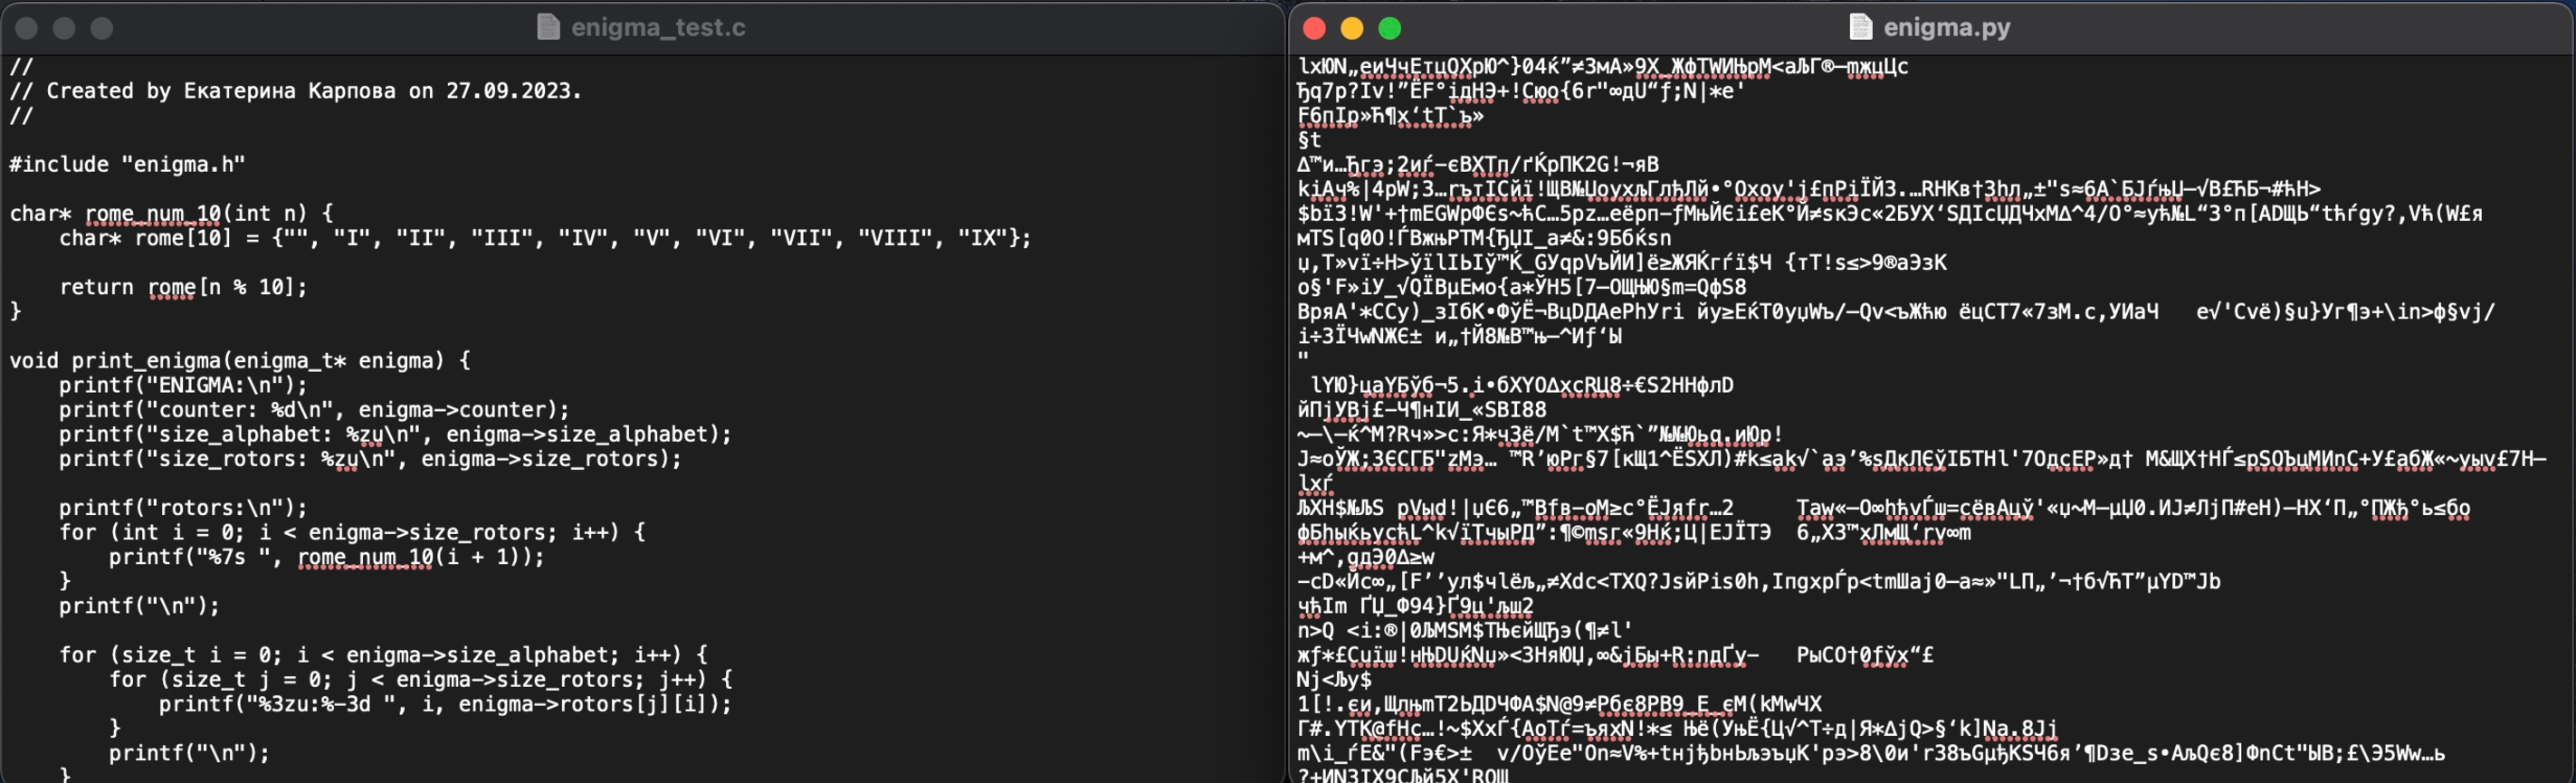
\includegraphics[width=0.9\linewidth]{inc/pdfs/6.pdf}
		\captionof{figure}{Файл исходного кода на языке C}
		\label{img:enigma}
	\end{tabular}
\end{table}

\begin{table}[H]
	\centering
	\begin{tabular}{p{1\linewidth}}
		\centering
		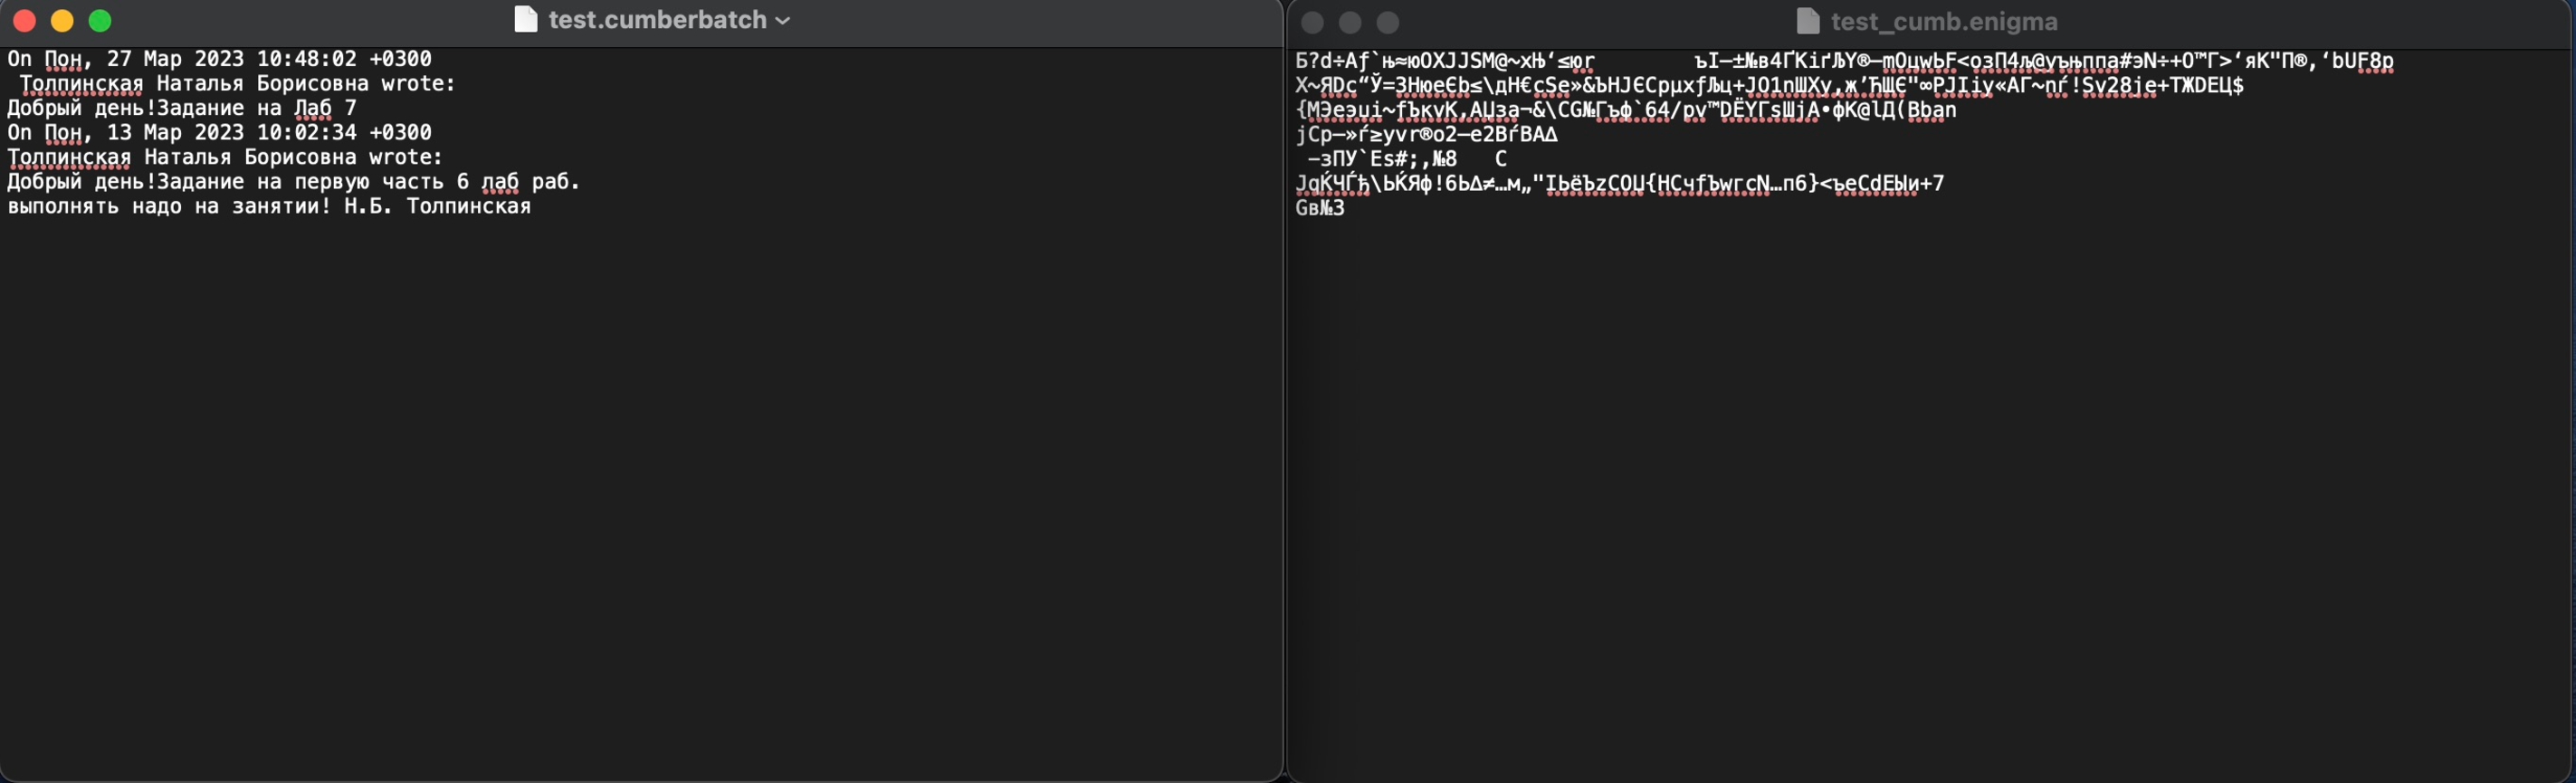
\includegraphics[width=0.9\linewidth]{inc/pdfs/7.pdf}
		\captionof{figure}{Файл с выдуманным расширением}
		\label{img:enigma}
	\end{tabular}
\end{table}

\begin{table}[H]
	\centering
	\begin{tabular}{p{1\linewidth}}
		\centering
		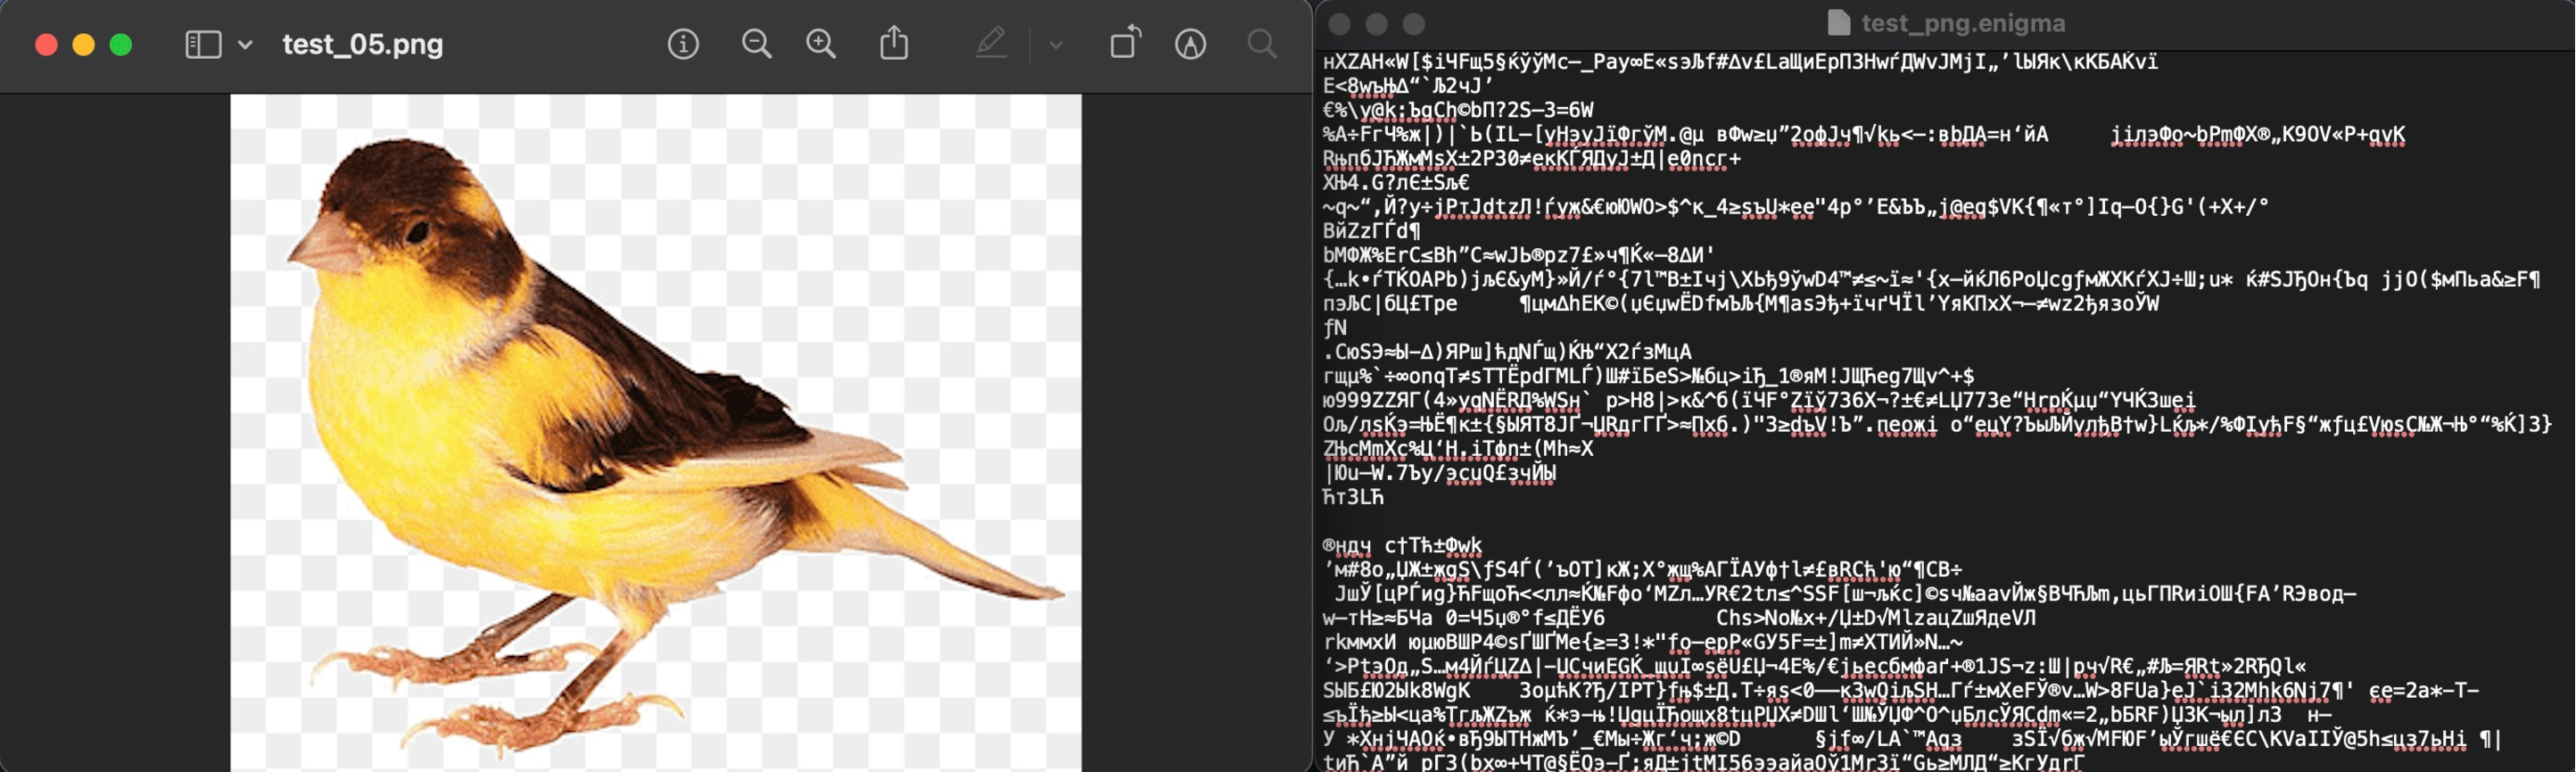
\includegraphics[width=0.9\linewidth]{inc/pdfs/8.pdf}
		\captionof{figure}{png изображение}
		\label{img:enigma}
	\end{tabular}
\end{table}
	
\end{appendices}
\begin{appendices}
\label{appendix:test-programs}

\chapter{Тестовые программы}

\includelistingpretty{program1}{}{Тестовая программа 1}

\includelistingpretty{program2}{}{Тестовая программа 2}

\includelistingpretty{program3}{}{Тестовая программа 3}

\includelistingpretty{program5}{}{Тестовая программа 4}
	
\end{appendices}
% \begin{appendices}
	\label{appendix:test-programs-res}
	
	\chapter{Тестовые программы c результатом на LLVM IR}
	
	\includelistingpretty{fibonacci}{}{Вычисление n-го числа Фибоначчи на Lua}
	
	\includelistingpretty{fibonacci_res}{}{Вычисление n-го числа Фибоначчи на LLVM IR}
	
	\includelistingpretty{fibonacci_recursive}{}{Вычисление n-го числа Фибоначчи с рекурсией на Lua}
	
	\includelistingpretty{fibonacci_recursive_res}{}{Вычисление n-го числа Фибоначчи с рекурсией на LLVM IR}

	\includelistingpretty{revert_list}{}{Инвертирование списка на Lua}
	
	\includelistingpretty{revert_list_res}{}{Инвертирование списка на LLVM IR}
		
\end{appendices}

\end{document}